\chapter{Auswertung}
Der HMF-Gehalt der Proben wird mit zwei Methoden bestimmt. Diese werden im folgenden Abschnitt vorgestellt, angewandt und miteinander verglichen. Außerdem wird die Genauigkeit der beiden Methoden über die Wiederfindungsrate überprüft.
\section{Kalibrierung}
Zur Bestimmung von HMF wird eine Kalibrierung durchgeführt. Um die Linearität des Messsignals bei verschiedenen Konzentrationen zu gewährleisten müssen mehrer Kalibrierlösungen vermessen werden. Da ein von 5 bis 300mg/kg großer Bereich abgedeckt werden soll fiel die Entscheidung auf sechs Messpunkte. Die Konzentrationen der Kalibrierstandard sind in folgender Tabelle aufgetragen:

\begin{table}[htbp]
	\centering
		\begin{tabular}{p{0.30\linewidth}|p{0.25\linewidth}|p{0.25\linewidth}|p{0.2\linewidth}}
			Standard & Extinktion & Konzentration / [mg/L] &  Massenanteil / [mg/kg]\\
			\hline
			Std 1 & 0,0400 & 1,004 & 5\\
			\hline
			Std 2 & 0,1353 & 3,032 & 15\\
			\hline
			Std 3 & 0,1687 & 5,020 & 25\\
			\hline
			Std 4 & 0,3214 & 10,040 & 50\\
			\hline
			Std 5 & 0,9453 & 30,320 & 152\\
			\hline
			Std 6 & 1,8987 & 60,640 & 303
		\end{tabular}
	\caption{Kalibrierungen}
	\label{tab:Kalibrierungen}
\end{table}

Die abgegebenen Gehalte und Konzentrationen beziehen sich auf eine theoretische Probeneinwaage von 10,0g Honig.\\
Trägt man nun die Kalibrierpunkte in einem Diagramm ein ergibt sich eine Gerade mit der Funktion y=0,0309*x+0,0175 bei einem Bestimmtheitsmaß von 0,9997.

\begin{figure}[htbp]
	\centering
		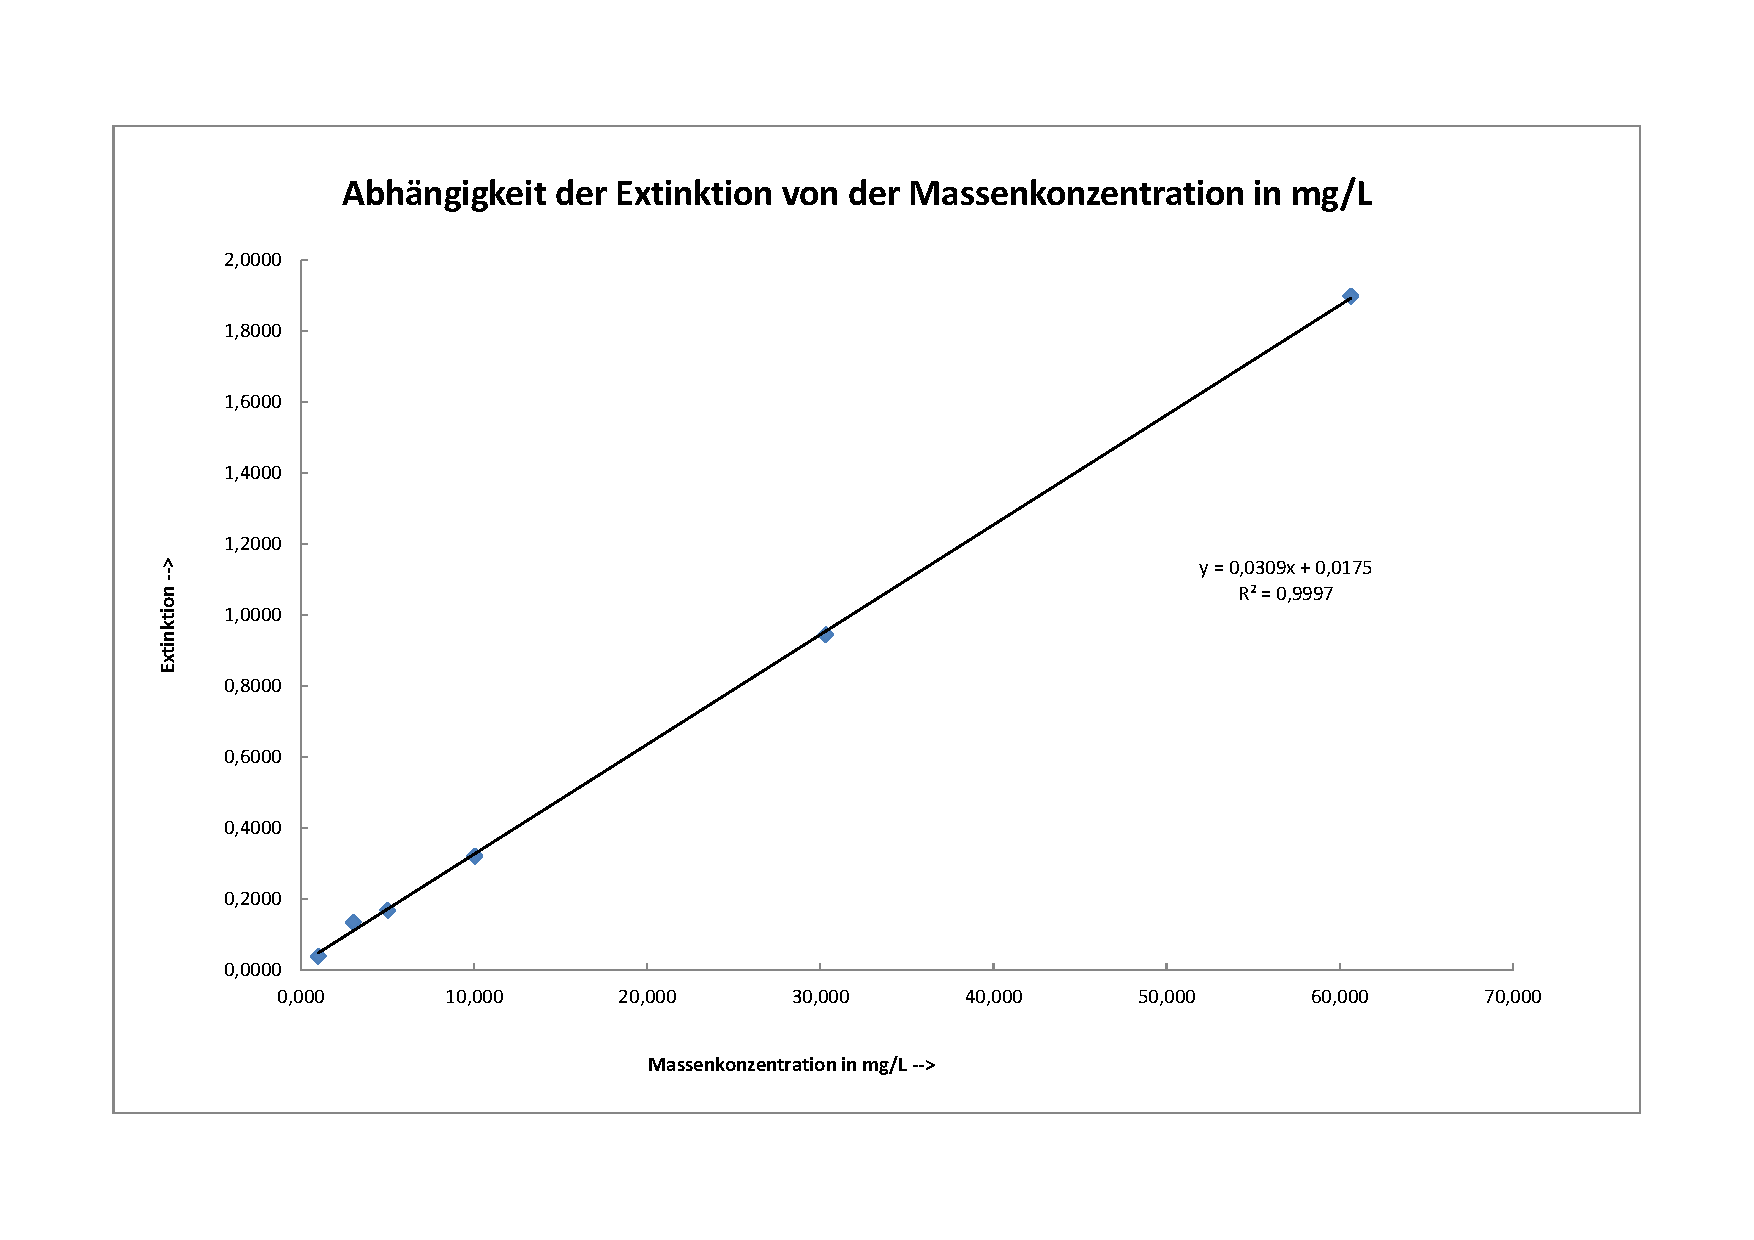
\includegraphics[width=\textwidth]{../../DiagrammKalibrierung.pdf}
	\caption{Kalibriergerade}
	\label{fig:DiagrammKalibrierung}
\end{figure}

%Diagramm mit Kalibriergeraden hier einfügen

\section{Quantifizierung mittels Kalibriergerade}
Die durch die Kalibrierung ermittelte Funktion wird zur Bestimmung des Analytgehalts verwendet.
	\[y=m*x+b\]
	\[y=0,0309*x+0,0175\]
	\[x=\frac{ y-0,0175 }{ 0,0309 }\]
Beispielrechnung zu Probe 3 (warm):
	\[x=\frac{ 1,9812-0,0175 }{ 0,0309 }\]
	\[x=63,55mg/L\]
Die Massenkonzentration muss nun noch in den Massenanteil umgerechnet werden.
	\[w[mg/kg]=\frac{ \beta*V }{ 1L * m }*1000000\]
	\[w[mg/kg]=\frac{ 0,06355g/L*0,05L }{ 1L * 10,041g }*1000000\]
	\[w[mg/kg]=316mg/kg\]

	
\section{Quantifizierung mittels Festfaktor}
In der Analysevorschrift zur Bestimmung von HMF in Honig ist folgende Formel angegeben:
	\[HMF[mg/kg]=\frac{ E * 1920 }{ m }\]
Hierbei steht E für die Extinktion, m für die Probenmasse und der Festfaktor 1920 setzt sich zusammen aus dem molaren Extinktionskoeffizienten und der Verdünnung und Umrechnung in die gewünschte Einheit mg/kg.
	\[Faktor=\frac{ M(HMF)*V }{ \epsilon }*1000000\]
	
	\[1920=\frac{ 126g/mol * 0,05L }{ 3,28125L/mol }*1000000\]
Beispielrechnung zu Probe 3 (warm):
	\[HMF[mg/kg]=\frac{ 1,9812 * 1920 }{ 10,041g }\]
	\[HMF[mg/kg]=379mg/kg\]
\section{Ergebnisse der analysierten Proben}
Alle Proben wurden mit den beiden zur Verfügung stehenden Methoden quantifiziert und in einer Tabelle aufgetragen.

\begin{table}[htbp]
	\centering
		\begin{tabular}{p{0.30\linewidth}|p{0.17\linewidth}|p{0.25\linewidth}|p{0.25\linewidth}} 
			Probenbezeichnung & Extinktion & Gehalt HMF über Kalibrierung \ [mg/kg] &  Gehalt HMF über Festfaktor \ [mg/kg]\\
			\hline
			1 Flotte Biene Frühlingsblütenhonig (kalt) & 0,016 & <5 & <5\\
			\hline
			1 Flotte Biene Frühlingsblütenhonig (warm) & 1,6041 & 256 & 307\\
			\hline
			2 Flotte Biene Gebirgsblütenhonig (kalt) & 0,0102 & <5 & <5\\
			\hline
			2 Flotte Biene Gebirgsblütenhonig (warm) & 1,3184 & 210 & 252\\
			\hline
			3 Sommerblütenhonig (kalt) & 0,1500 & 20 & 27\\
			\hline
			3 Sommerblütenhonig (warm) & 1,9812 & 316 & 379\\
			\hline
			4 Blütenhonig (kalt) & 0,0621 & 7 & 12\\
			\hline
			4 Blütenhonig (warm) & 1,5500 & 245 & 294\\
			\hline
			5 Mexico (kalt) & 0,0639 & 8 & 12\\
			\hline
			5 Mexico (warm) & 1,2237 & 194 & 234\\
			\hline
			6 Ägäis (kalt) & 0,0871 & 11 & 16\\
			\hline
			6 Ägäis (warm) & 1,1639 & 185 & 223\\
			\hline
			7 Waldhonig & 0,0362 & <5 & 7\\
			\hline
			8 Zuckerrübensirup & n.B. & n.B. & n.B.\\
			\hline
			9 Winterfutter & 0,0255 & <5 & 5\\
			\hline
			10 Invertzucker & 1,541 & 249 & 298\\

		\end{tabular}
	\caption{Messergebnisse}
	\label{tab:Messergebnisse}
\end{table}

\section{Wiederfindungsrate}
Da zur Bestimmung des HMF-Gehalts nur ideale Kalibrierlösungen bzw. der angegebene Festfaktor verwendet wurden, muss der Einfluss der Probenmatrix auf das Analysenergebnis ermittelt werden. Hierzu wird die Wiederfindungsrate anhand einer Aufstockung ermittelt. Die Wiederfindungsrate (WFR) ist der Quotient aus dem Istwert und dem Sollwert der Probe. Zur Berechnung der Wiederfindung wird die folgende Formel verwendet:
	\[WFR=\frac{ Gefundener Gehalt + Istwert }{ Gefundener Gehalt + Sollwert } *100 \]
Als Gefundener Gehalt wird der Mittelwert aus der Sechsfachbestimmung der Probe 3 verwendet.
	\[x(Mittelwert)=\frac{ x1+x2...xn }{ n } \]
Die Berechnung des Mittelwertes nach dem in der Vorschrift angegeben  Festfaktor:
	\[28mg/kg=\frac{ 29mg/kg+31mg/kg+25mg/kg+25mg/kg+31mg/kg+28mg/kg }{ 6 } \]
Die Berechnung des Mittelwertes nach der erstellten Kalibriergerade:
	\[21mg/kg=\frac{ 22mg/kg+23mg/kg+18mg/kg+19mg/kg+23mg/kg+21mg/kg }{ 6 } \]
Nach dem gemittelten Gehalt muss der aufgestockte Anteil an Analyt berechnet werden. In eine Aufstockung wurden 10ml der Stammlösung 1.1 zugegeben. Das entspricht einer Masse von 0,502 mg. Bezogen auf die Probeneinwaage von 10,483g ergibt sich ein theoretischer Massenanteil von:  
	\[w=\frac{ m(Analyt) }{ m(Gesamt) } \]
	\[47,9mg/kg=\frac{ 0,502mg }{ 0,010483kg } \]
In einer zweiten Aufstockung wurden 5ml Stammlösung 2.1 zugegeben, was einer Masse von 0,758mg entspricht. Auch hier wird mit der Einwaage von 10,365g der theoretische Massenanteil berechnet:
	\[73,1mg/kg=\frac{ 0,758mg }{ 0,010365kg } \]
Mit den Mittelwerten und den theoretischen kann die Wiederfindungsrate berechnet werden.\\
Zuerst die erste Aufstockung anhand des Festfaktors:
	\[92,3=\frac{ 28mg/kg + 47,9mg/kg }{ 82mg/kg } *100 \]
Und nach der Kalibriergeraden:
	\[104,4=\frac{ 21mg/kg + 47,9mg/kg }{ 66mg/kg } *100 \]
Anhand der beiden Wiederfindungsraten kann man darauf schließen, dass die Quantifizierung mit der Kalibriergeraden richtigere Werte liefert. Zur Kontrolle werden beide Berechnungen noch einmal mit der zweiten Aufstockung durchgeführt.\\
Bestimmung der zweiten Aufstockung nach Festfaktor:
	\[95,4=\frac{ 28mg/kg + 73,1mg/kg }{ 106mg/kg } *100 \]
Bestimmung der zweiten Aufstockung nach Kalibriergeraden:
	\[108,2=\frac{ 21mg/kg + 73,1mg/kg }{ 87mg/kg } *100 \]
Beide Wiederfindungsraten sind nahe 100 \% jedoch findet man mit der Kalibriergeraden tendenziell leicht erhöhte Gehalte an HMF wieder, während man in den Proben weniger HMF findet. Es ist auch bemerkenswert wie gut der angegebene Festfaktor zur Gehaltsbestimmung geeignet ist obwohl bei seiner Verwendung in keinster Weise kalibriert wird und das verwendete Messgerät damit völlig ignoriert wird. Auch bei der Richtigkeit der Ergebnisse sind beide Methoden vergleichbar.
	
\section{Standardaddition}
Da die Probe 3 zweimal mit unterschiedlichen Mengen an HMF aufgestockt wurde bietet sich ein Quantifizierung über Standardaddition an. So lässt sich auch der Einfluss der, nach der Abtrennung noch enthaltenen, Probenmatrix eliminieren. Eine Übereinstimmung mit unseren anderen Ergebnissen würde für einen nur Unwesentlichen Einfluss der verbliebenen Matrixanteile sprechen. Der Massenanteil mit mehreren Aufstockungen wird berechnet in dem man die Extinktion der Probe(hier die Mittelwerte der sechs Bestimmungen von Probe 3) sowie die Extinktionen der Aufstockungen zur Erstellung eines Diagramms verwendet. Die Probe ohne Aufstockung markiert den Nullpunkt der X-Achse, jede Aufstockung ist auf der X-Achse gemäß ihrer zugesetzten Konzentration aufgetragen. 
%Diagramm hier einfügen
Zieht man durch die erhaltenen Punkte eine Gerade und verlängert sie zurück bis sie die X-Achse im negativen Bereich schneidet, kann man an diesem Punkt die Konzentration der Probe graphisch ablesen. Der Gehalt der Probe lässt sich zudem über die lineare Regression der Geraden bestimmen. Sie lautet bei dieser Analyse:
	\[y=0,0058*x+0,1572\] 
Setzt man y nun gleich 0 und löst nach x auf erhält man die Konzentration der Probe in mg/kg.
 	\[0=0,0058*x+0,1572\] 
	\[x=\frac{ -1,572 }{ 0,0058 }   |*-1\] 
	\[x=27mg/kg\] 
Der über Standardaddition ermittelte Gehalt an HMF in der Probe 3 ist damit 27mg/kg und entspricht damit praktisch dem Gehalt der mit den anderen Quantifizierungsmethoden ermittelt wurde.